The Interactive Graph Cuts aglorithm, developed by Boykov and Jolly \cite{graphCuts} uses a CRF for interactive image segmentation. The regional penalty term can be computed from user input. Once the user has marked some pixels as part of the object and some as part of the background, 2 histograms of grayscale values can be computed, from which probability values can be computed and penalties inferred.

\begin{figure}[h!]
\centering
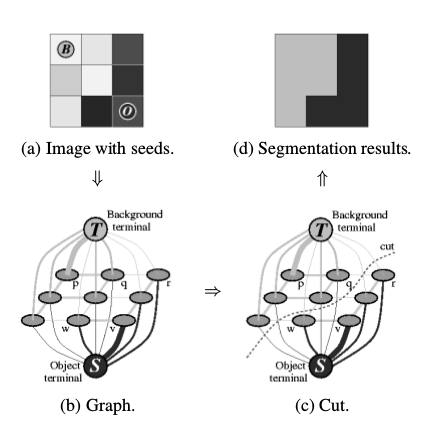
\includegraphics[scale=0.55]{pictures/graphCuts}
\caption{Image showing the process for the graph cuts algorithm for a 3x3 image. Nodes $p$ and $v$ have been marked by the user as background and object respectively. The cost of each weight is represented by it's thickness, and the minimum cut will prefer inexpensive edges. The edges between pixels represent boundary terms, and those between a pixel and a terminal represent the regional term for that terminal. \cite{graphCuts}}
\label{fig:graphCut}
\end{figure}

Including interactivity is a minor tweak: if a user sets a pixel $(i,j)$ to binary value $l$, then $R_{i,j,\neg k} = \delta_{k,l} K$, with $K = 1 + B _\text{max}$ where $B_{\text{max}}$ is the largest value of the boundary term for a single pixel. This guarantees that pixels sets by the user will be set correctly in the output, giving them more importance in the graph. The segmentation is found using a minimum cut algorithm as described earlier (see figure \ref{fig:graphCut}). 

Graph cuts offers some possibility of learning, by building histograms of historic data as more and more segmentation is done. However, this form of learning is relatively simple compared to CNNs, which can learn much more complex spatial relationships. It is likely that it would generalize to unseen data much more poorly than a CNN would.